
\documentclass[9pt,sigconf]{acmart}

\usepackage{color}
\usepackage{graphicx}
%\usepackage[justification=centering]{caption}
%\usepackage{subcaption}
%\usepackage{cite}


\usepackage{amssymb,amsmath}
%\renewcommand{\baselinestretch}{1.0}
%\setlength\floatsep{1pt plus 0.5pt minus 0.5pt}
%\setlength\textfloatsep{0pt plus 1pt minus 1pt}

\makeatletter
\def\hlinewd#1{%
\noalign{\ifnum0=`}\fi\hrule \@height #1 %
\futurelet\reserved@a\@xhline}
\makeatother
\usepackage{booktabs}
\usepackage{multirow}

\usepackage[binary-units=true]{siunitx}

%\usepackage[algoruled,noline,longend,linesnumbered]{algorithm2e}
%\setlength{\algomargin}{2.5em}
%\SetNlSkip{1.2em}
%\SetNlSty{textbf}{L}{}

\makeatletter
\def\hlinewd#1{%
  \noalign{\ifnum0=`}\fi\hrule \@height #1 %
\futurelet\reserved@a\@xhline}
\makeatother
\usepackage[tworuled,noline,linesnumbered]{algorithm2e}
\setlength{\algomargin}{2.0em}
\SetNlSkip{0.9em}
\SetNlSty{textbf}{L}{}
\SetAlFnt{\footnotesize}
\SetAlCapFnt{\footnotesize}
\SetAlCapNameFnt{\footnotesize} 


\usepackage{pgfplots}
\usepackage{pgfplotstable}
\usepackage{siunitx}
%\usepackage{tikz}


%\setlength\thinmuskip{0mu}
\setlength\medmuskip{3mu}
%\setlength\thickmuskip{0mu} 

%subparagraph not defined in IEEEtran but needed by titlesec
%\usepackage[compact]{titlesec}
%\titlespacing{\section}{0pt}{8pt}{2pt}
%\titlespacing{\subsection}{0pt}{6pt}{2pt}
%\titlespacing{\section}{0pt}{2pt}{1pt}
%\titlespacing{\subsection}{0pt}{2pt}{1pt}



%\setlength{\abovedisplayskip}{2pt plus 1pt minus 1pt}
%\setlength{\abovedisplayshortskip}{1pt plus 1pt minus 0.5pt}
%\setlength{\belowdisplayskip}{2pt plus 1pt minus 1pt}
%\setlength{\belowdisplayshortskip}{1pt plus 1pt minus 0.5pt}
\setlength\floatsep{10pt plus 0.5pt minus 0.5pt}
%\setlength\dblfloatsep{10pt plus 0.5pt minus 0.5pt}
%\setlength\intextsep{1pt plus 0.5pt minus 0.5pt}
\setlength\textfloatsep{3pt plus 1pt minus 1pt}
%\setlength\dbltextfloatsep{1.5pt plus 1pt minus 1pt}
\setlength\abovecaptionskip{3pt plus 0.5pt minus 0.5pt}
\setlength\belowcaptionskip{1pt plus 0.5pt minus 0.5pt}

%\makeatletter
%%change spaces around equations in amsmath
%\g@addto@macro\normalsize{%
  %\setlength\abovedisplayskip{2.8pt}
  %\setlength\belowdisplayskip{2.8pt}
  %\setlength\abovedisplayshortskip{-7.5pt}
  %\setlength\belowdisplayshortskip{0.8pt}
%}
%\makeatother

\setlength\evensidemargin{-2.3pc}
\setlength\oddsidemargin{-2.3pc}
\setlength\topmargin{-3.7pc}                % Nominal distance from top of
%%page to top of
%\textheight 666pt   %%original    % 9 1/4 column height
\setlength\textheight{689pt}
%\textwidth 42pc     %%original    % Width of text line.
\setlength\textwidth{43.8pc}         % Width of text line.
%\setlength\topmargin{-5.5pc}
%\setlength\columnsep{1pc}         %    Space between columns
\setlength\columnsep{1pc}         %    Space between columns

%
%%\makeatletter % access to internal commands
%%\renewcommand{\@seccntformat}[1]{\csname the#1\endcsname\ }
%%%\makeatother

%\setcounter{page}{1}
%\pagestyle{fancy}
%\renewcommand{\headrulewidth}{0pt}
%\fancyhf{}
%\rfoot{\small \thepage/\pageref{LastPage}}
%\rhead{\small \thepage}
%\setcopyright{acmcopyright}

%\setcopyright{rightsretained}
\settopmatter{printacmref=false} % Removes citation information below abstract
%\renewcommand\footnotetextcopyrightpermission[1]{} % removes footnote with conference information in first column
%\pagestyle{plain} % removes running headers


\copyrightyear{2018}
\acmYear{2018}
\setcopyright{acmcopyright}
\acmConference[DAC '18]{DAC '18: The 55th Annual Design Automation Conference 2018}{June 24--29, 2018}{San Francisco, CA, USA}
\acmBooktitle{DAC '18: DAC '18: The 55th Annual Design Automation Conference 2018, June 24--29, 2018, San Francisco, CA, USA}
\acmPrice{15.00}
\acmDOI{10.1145/3195970.3196025}
\acmISBN{978-1-4503-5700-5/18/06}

\begin{document}

%\frontmatter
%\pagestyle{headings}
%\pagestyle{plain}


\graphicspath{{Fig/}}
\def\figname{Figure}
\def\algname{Algorithm}
%\def\algname{Procedure}
%\newcommand{\figurefontsize}{\fontsize{7.0pt}{1}\selectfont}
\newcommand{\figurefontsize}{\small}

\pagestyle{empty}

\begin{abstract}

Flow-based microfluidic biochips have attracted much attention in the EDA community due to their miniaturized size and execution efficiency. Previous research, however, still follows the traditional
computing model with a dedicated storage unit, which actually becomes a bottleneck of the performance of biochips. In this paper, we propose a distributed channel-storage architecture (DCSA) to cache fluid samples inside flow channels temporarily.
Since distributed storage can be accessed more efficiently than a dedicated storage unit and channels can switch between the roles of transportation and storage easily, biochips with this architecture can achieve a higher execution efficiency even with fewer resources. Furthermore, we also address the flow-path planning that enables the manipulation of actual fluid transportation/caching on a chip. Simulation results confirm that the execution efficiency of a bioassay can be improved by up to 28\%, while the number of valves in the biochip can be reduced significantly. Also, flow paths for transportation tasks can be constructed and planned automatically with minimum extra resources.

\begin{IEEEkeywords}
Microfluidic biochips, channel storage, scheduling, architectural synthesis, flow-path mapping.
\end{IEEEkeywords}

\end{abstract}


\newcommand{\papertitle}{Design-for-Testability for Continuous-Flow Microfluidic Biochips}


\title{\papertitle}
%\author{
%  \vskip 10pt
 %Chunfeng Liu$^1$, Bing Li$^1$, Bhargab B. Bhattacharya$^2$, Tsung-Yi
%Ho$^{34}$, Ulf Schlichtmann$^1$\\
%$^1$Institute for Electronic Design Automation, Technical University of Munich (TUM), Munich, Germany\hfill\\
%$^2$Indian Statistical Institute, Kolkata, India\hspace{18pt}
%$^3$National Tsing Hua University, Hsinchu, Taiwan \hfill\\
%$^4$Institute for Advanced Study, Technical University of Munich (TUM), Garching, Germany\hfill
%}
%\author{}
%\institute{}
%\vskip 50em

\author{
Chunfeng Liu$^{1,4}$, Bing Li$^1$, 
Tsung-Yi Ho$^{2,4}$, 
Krishnendu Chakrabarty$^{3,4}$, 
Ulf Schlichtmann$^1$\\
\normalsize 
$^1$Chair of Electronic Design Automation, Technical University of
Munich, Germany\hskip 10pt $^2$National Tsing Hua University, Hsinchu, Taiwan \\
$^3$Department of ECE, Duke University, Durham, NC, USA \hskip 10pt 
$^4$Institute for Advanced Study, Technical University of Munich, 
Germany\\
\{chunfeng.liu, b.li, ulf.schlichtmann\}@tum.de, tyho@cs.nthu.edu.tw, krish@ee.duke.edu
}



\maketitle




% this file is called up by thesis.tex
% content in this file will be fed into the main document

%: ----------------------- introduction file header -----------------------
\chapter{Introduction}

% the code below specifies where the figures are stored
\ifpdf
    \graphicspath{{1_introduction/figures/PNG/}{1_introduction/figures/PDF/}{1_introduction/figures/}}
\else
    \graphicspath{{1_introduction/figures/EPS/}{1_introduction/figures/}}
\fi

% ----------------------------------------------------------------------
%: ----------------------- introduction content ----------------------- 
% ----------------------------------------------------------------------



%: ----------------------- HELP: latex document organisation
% the commands below help you to subdivide and organise your thesis
%    \chapter{}       = level 1, top level
%    \section{}       = level 2
%    \subsection{}    = level 3
%    \subsubsection{} = level 4
% note that everything after the percentage sign is hidden from output



\section{The rise of the chip} % section headings are printed smaller than chapter names
% intro

The field of microfluidics has four parents: molecular analysis, biodefence, molecular biology and microelectronics. 
First came analysis. The distant origins of microfluidics lie in microanalytical methods — gas-phase chromatography (GPC), 
high-pressure liquid chromatography (HPLC) and capillary electrophoresis (CE) — which, in capillary format, revolutionized chemical analysis. These methods (combined with the power of the laser in optical detection) made it possible to simultaneously achieve high sensitivity and high resolution using very small amounts of sample. With the successes of these microanalytical methods, it seemed obvious to develop new, more compact and more versatile formats for them, and to look for other applications of microscale methods in chemistry and biochemistry. A second, different, motiva

The first key area that inspired the field of microfluidics is molecular analysis. 

A second, different, motivation for the development of microfluidic systems came with the realization — after the end of the cold war — that chemical and biological weapons posed major military and terrorist threats. To counter these threats, the Defense Advanced Research Projects Agency (DARPA) of the US Department of Defense supported a series of programmes in the 1990s aimed at developing field-deployable microfluidic systems designed to serve as detectors for chemical and biological threats. These programmes were the main stimulus for the rapid growth of academic microfluidic technology.

The third motivational force came from the field of molecular biology. The explosion of genomics in the 1980s, followed by the advent of other areas of microanalysis related to molecular biologies, such as high-throughput DNA sequencing, required analytical methods with much greater throughput, and higher sensitivity and resolution than had previously been contemplated in biology. Microfluidics offered approaches to overcome these problems. The fourth contribution was from microe


The original hope of microfluidics was that photolithography and associated technologies that had been so successful in silicon microelectronics,
[The origins and the future of microfluidic]


Microfluidic biochips are revolutionizing the traditional biochemical experiment 
flow with their high execution efficiency and 
miniaturized fluid manipulation \cite{JEMP08, EVNR03,JMSQ07}. 
Devices are built 
%from microchannels and valves 
in such a chip to execute specific operations, such as mixing and detection.
Fluid samples are transported through microchannels between devices to carry
out the protocol of a bioassay. 
All these functions are performed at the nanoliter level and
controlled by a microcontroller without human intervention. 
The efficiency and reliability of such miniaturized and automated chips 
endow them with a great potential to improve human life significantly, 
and the research to bridge them with real-world applications
%bring them from prototypes in laboratories to industry production 
is key to their success.   

\begin{figure}[htpb]
    {      
    \centering
    % \input{Fig/valve_mixer_chip.pdf_tex}
    \input{1_introduction/figures/valve_mixer_chip.pdf_tex}
    %\includegraphics{Fig/valve_mixer_chip.png}
    \caption{Components and structure of flow-based biochips. 
    (a) Valves constructed at intersections of flow/control channels \cite{JMSQ07}. 
    (b) Mixer \cite{JMSQ07}. (c) A part of a biochip
    containing a mixer surrounded by a transportation channel network 
    \cite{ESWD13}.}
    \label{fig:valve_mixer_chip}
    }
    \end{figure}

A flow-based microfluidic biochip is constructed from basic components such as
%basic components, namely, 
microchannels and microvalves, henceforth named as channels and valves for
simplicity.
Flow channels are used to transport reaction samples and reagents
between different locations. Above flow channels, control 
channels are built to 
conduct air pressure to intersections of flow channels and control channels 
to form 
valves, as illustrated in \figname~\ref{fig:valve_mixer_chip}(a),
where three valves are constructed at the intersections.
These channels are built from elastic materials, so that
air pressure in a control channel can block the movement of fluid sample
by squeezing the flow channel downwards.
Conversely, if the pressure in the control channel is
released, the fluid sample can resume its movement. 
%Functionally, valves are thus formed at intersections of
%flow channels and control channels, and the open/close states
%of valves are controlled by the air pressure fed into the 
%control channels. 
Since the channel width has been miniaturized
down to 50 um \cite{Studer04} thanks to the advance of manufacturing
technology, a huge number of channels and valves can
already be integrated
into a single biochip to perform large-scale experiments and diagnoses.

With valves as basic controlling components, complex devices 
can be constructed. For example, mixers can be built using
channels and valves to execute mixing operations, which are very
common in biochemical applications. The structure of a mixer is shown
in \figname~\ref{fig:valve_mixer_chip}(b),
where the three valves at the bottom are actuated alternately by 
applying and releasing air pressure in the control
channels 
%to form a circular flow around the device 
to mix fluid samples and reagents by peristalsis.
The execution of a mixing operation in a biochip is demonstrated
in a video \cite{mixing_store}. 
After the mixing operation is completed, the resulting fluid sample 
can be stored in a dedicated storage unit temporarily. %in the biochip.

In a biochip, devices executing specific operations, e.g., mixing and heating,
are connected by channels so that intermediate reaction results %fluid samples 
can be
transported between devices for processing. All these operations and
transportation are controlled
%by valves, whose open/close states are regulated
by a microcontroller, which 
%. To execute a biochemical assay, the microcontroller 
issues instructions in a given order to actuate valves 
to move fluid samples 
%between devices 
and execute operations.
%of valve actuation to move fluid samples
%to different devices to process them. 
%The photograph of a complete biochip is
%shown 
\figname~\ref{fig:valve_mixer_chip}(c) shows a mixer (reaction loop) surrounded
by flow channels (green), control channels (yellow and red) and valves
(yellow and red blocks).
%formed 
%at their
%At the 
%intersections.
%of flow and control channels, 
%used to direct fluid transportation. 
These channels and valves together form a network similar to the
road transportation system. If fluid channels should cross, %four
valves are built %at the crossing point 
to form a switch, as shown 
in \figname~\ref{fig:valve_mixer_chip}(c).
At any moment, only two out of the four valves should be opened to 
direct fluid transportation; 
%form a flow path; 
the other two valves must be closed to avoid fluid
contamination. Consequently, the role of the valves at the intersection
of %two 
flow channels is similar to that of the traffic lights in the road
transportation system, while the open/closed states of the valves are
controlled by a microcontroller according to the protocol of the application.
%and many valves are used to coordinate fluid
%transportation and assay execution. 
The mixer and the channel network
%The size of the chip in 
in \figname~\ref{fig:valve_mixer_chip}(c)
are implemented into a biochip of the size comparable to that of a coin 
as shown %in the photo 
at the upper left
corner, %of \figname~\ref{fig:valve_mixer_chip}(c), 
demonstrating the miniaturized integration of 
microfluidic biochips. 


\begin{figure}
    {
    \vskip -5pt
    \figurefontsize
    \centering
    \input{1_introduction/figures/sequencing_graph.pdf_tex}
    \caption{Sequencing graph of a bioassay.}
    \label{fig:sequencing_graph}
    }
    \end{figure}

    In a biochip, the open/closed states of valves and the transportation of
fluid samples are determined according to the biochemical application executed by the
biochip. A biochemical application, or \textit{bioassay} henceforth,  
%A biochemical application, or a bioassay, 
is usually described with
%describes the operations 
%executed by a biochip and their dependency with 
a \textit{sequencing graph} $\mathcal{G}=(\mathcal{O},\mathcal{E})$, such as in
\figname~\ref{fig:sequencing_graph}, where $\mathcal{O}$ is
the set of nodes %representing operations,
and $\mathcal{E}$ is the set of edges. %in the graph specifying the dependency
%relation between operations. 
A node $O_i \in \mathcal{O}$ in the sequencing graph
represents an operation, whose type $\tau_i$ and duration $u_i$ are specified by the user.
The type $\tau_i$ of the operation, e.g., mix, heat and filter, is predefined by the application. 
To execute an operation, the corresponding device must be built in the chip
and the operation must be assigned to this device.
An edge $e_{ij}\in \mathcal{E}$ from $O_i$ to $O_j$
in the sequencing graph specifies that $O_i$ must be executed before $O_j$ and the 
result of $O_i$ is the input of $O_j$. If $O_i$ and $O_j$ are executed by
different devices, the required fluid transportation must be performed by the channel
network between devices. 

Biochips have a huge advantage over the traditional manual experiment
flow, where operations performed by humans are error-prone 
and inaccurate.  Any inadvertent mistake in this manual process 
might ruin a complex experiment that may
last for several days. In a biochip, the volumes of fluid samples and reagents are
controlled accurately and fluid samples are moved to target devices reliably,
%because the whole experiment is controlled 
%all of which are managed
all of which are managed
by a microcontroller exactly following a
given protocol.
In addition, the miniaturized size of biochips makes them
extremely portable, so that a complex lab can be integrated into a single chip
and carried conveniently to perform on-the-spot tests to counter acute 
disease outbreaks 
such as the devastating Ebola virus disease a few years ago.
Furthermore, reactions with fluid samples and reagents of tiny volumes
take less time to complete than those with large volumes in tubes and
in the traditional experiment flow, so that biochips are also more
responsive in dealing with urgent situations.
Moreover, %Economically, 
biochips save precious reagents by performing operations at
nanoliter level. %The required 
%Such reagents may be exorbitantly expensive. 
For example, RNase inhibitor, a polyclonal antibody
commonly used in reverse transcription polymerase chain reaction, cost 600 euros per milliliter in December 2014 
\cite{RNasePrice}. 

The miniaturization of microfluidic biochips also has the potential of
large-scale
system integration. Already in 2008, a biochip array with 25K valves was
accomplished \cite{JMPK08}, and recent advances in manufacturing technologies have 
led to
%enabled
a valve density of 1 million per cm$^2$ %\si{\square\centi\metre} 
\cite{C2LC40258K}. 
A system integration of this scale
enables long-aspired exhaustive diagnoses in identifying the illness 
of a patient by testing pathological samples with thousands of reagents 
simultaneously. This breakthrough will not only reduce
the inaccuracy in medical diagnoses, where individual expertise and experience
of doctors play an important role, but also change the current 
guess-then-test model of medical treatment. 
In addition, such exhaustive diagnoses can be performed in
small health-care centers routinely, 
due to the
tremendously miniaturized chip size and lowered cost. 
With this exhaustive diagnosis model, illnesses can be detected at a very early stage and 
treatment cost can be reduced significantly as well.

Owing to their efficiency and cost-effectiveness, microfluidic biochips are
reshaping many fields such as pharmacy, biotechnology and health care.
%in academic research as well as in applications.
In recent years, genomic bioassay protocols, such as nucleic-acid
isolation, DNA purification and DNA sequencing, have been successfully
demonstrated with microfluidic biochips. In addition, this technology has 
attracted a lot of commercial attention, e.g., from Illumina \cite{illum}, 
a market leader in DNA sequencing. 
%Furthermore, 
Accordingly, 
%%Recently,
%Frost \& Sullivan has estimated that the European lab-on-chip and microfluidics market 
%reaches about 1.62 billion USD even at the early growth phase of this
%technology. Correspondingly, 
the International Technology Roadmap
for Semiconductors (ITRS) 2015 \cite{itrs}
has  
%listed medical applications as one of application drivers and 
recognized the importance of microfluidic devices as 
having a rapid growth in the next several years. 

%Due to the importance of microfluidic biochips to human life and the huge
%potential market, research on microfluidic biochips has been growing
%continuously recently. Scientific papers have been published, e.g.,
%%in IEEE Trans. on CAD and in ACM J. on Emerg.  Tech.
%in IEEE Transactions on Computer-Aided Design of Integrated Circuits and
%Systems and ACM Journal on Emerging Technologies in Computing.
%Several renowned universities, for instance, CMU and Duke, have initiated research
%projects on design automation for microfluidic biochips. 
%Accordingly,
%at the Technical University of Munich,  with the support of the Institute for
%Advanced Study, funded by the German Excellence Initiative and
%the European Union Seventh Framework Programme, we have also established a
%research group focusing on design automation and optimization of microfluidic
%biochips. %at micro and macro level.


%\vskip 8pt
\textit{\underline{Synthesis of microfluidic biochips  using
computer algorithms}}


In a biochip, 
%it is very rare to assign each operation to a dedicated device 
%for cost reasons.
%Instead, 
operations are executed by a given number of devices with time
multiplexing,
%. Consequently, the execution of operations is 
described 
as
a schedule. For example, an execution %of the operations 
of the bioassay
illustrated in \figname~\ref{fig:sequencing_graph} is shown 
in \figname~\ref{fig:biochip_synthesis}(a), 
where two mixers, one heater, one filter, and one detector are available.
%This schedule, however, can still be improved by executing 
%$O_3$, $O_4$ and $O_6$ before $O_1$ and $O_2$ to produce fluid samples
%processed by $O_8$ and $O_9$ earlier. 
%Since the latter two operations use heater and filter instead of mixers, an
%early result from $O_6$ increases the parallelism of operation execution
%and thus shortens the overall execution time of the bioassay. 
%In the last step of synthesis, 
According to the schedule, 


\begin{figure}
    {
    \vskip -3pt
    \figurefontsize
    \centering
    \input{1_introduction/figures/biochip_synthesis.pdf_tex}
    \caption{Synthesis of microfluidic biochips.
    (a) Scheduling. (b) Physical design.}
    \label{fig:biochip_synthesis}
    }
    \end{figure}

    the layout of a biochip, 
    including the locations of devices and the transportation channels between them,
    can be determined to generate a physical design, 
    as shown in \figname~\ref{fig:biochip_synthesis}(b), where the devices
    are connected by a channel network controlled by valves.
    
    The synthesis process above demonstrates that the schedule of operations of a
    bioassay determines the overall execution time. 
    %In addition, the communication
    %between devices also affects the channel network for fluid transportation.
    In addition, the fluid transportation between devices 
    affects the structure of the channel network.
    Consequently, a holistic design automation flow is required to bridge the
    low-level components introduced by the microfluidics community with high-level
    real-world applications. In each step of this design automation flow, various design
    objectives should be optimized to achieve an efficient architecture for the
    biochip.
    
    The synthesis flow of biochips
    %shown in \figname~\ref{fig:biochip_synthesis} 
    is similar
    to the synthesis flow for integrated circuits \cite{Micheli94}. Therefore,
    researchers in the electronic design automation community have started to expand
    into this area in recent years \cite{ChakrabartyFZ10,PopAC15}. 
    However, these research efforts 
    %on flow-based biochips is 
    are still in an early stage and many unique characteristics of microfluidic
    biochips have still not been considered. %to date. 
    %problems need to be solved soon to pave the way for industry production
    %of biochips. 
    %are open. %still unsolved.
    
    \vskip 8pt
    \textit{\underline{Flow-based microfluidic architectures: the electronic view}}
    
    In the microfluidics community, researchers are focusing on developing new
    technologies and new structures to build fundamental components and devices,
    such as valves and pumps
    \cite{Unger113,mathies2010multiplexed}.
    Prototype microfluidic biochips are also built very often %, but usually 
    %for the purpose of 
    to demonstrate the function and performance of new
    components and new devices.
    %Besides new devices, 
    Another major focus of the microfluidics community is to
    increase the integration density of basic components. With the advance in MEMS
    technology, a large number of components such as valves can now be built in a
    single biochip \cite{C2LC40258K}. 
    Unfortunately, the abundant available resources 
    %from the advance in the microfluidc community
    have mostly been left unexplored, because end users cannot use them 
    without a system layer that presents an interface for user applications,
    similar to the scenario that an operating system is missing 
    for computer users. On the other hand, 
    %the lack
    %of applications has disheartened the microfluidics research community and
    %consequently their effort 
    the effort of the microfluidics research community
    has been spread out in exploring even 
    more technologies for microfluidic biochips, 
    %all of small size, 
    %while ignoring the potential of large system integration which 
    %they already have in hand.
    leading to a flourishing but fragmented panorama in the research on
    microfluidics. 
    
    The %state of the art in 
    status of
    the microfluidics community is similar to the early
    period of the semiconductor industry. At that time, researchers
    were exploring different materials and device structures to build smaller but
    faster transistors. Thereafter, CMOS-based technology became dominant
    in this industry, while other technologies are 
    employed only for specific applications. 
    CMOS technology obtained its dominance because of
    %, first of all, 
    its performance. 
    %However, a very important factor which assisted this dominance is that
    %the semiconductor industry and the electronic design automation community  
    %have found a way to carry out mass production of these devices and shrink the
    %feature size continuously. 
    However, the development of Electronic Design Automation (EDA) has 
    supported the large-scale integration in design and manufacturing and
    %, while  
    %with smaller devices, 
    %In the meantime,
    %Moreover, 
    %the computer community has developed a successful computing model
    %to 
    %also presented the available resources to 
    %%end users 
    %%and facilitate the development of 
    %high-level applications successfully.
    made the computing resources available to designers successfully.
     
    Observing the state of the art of microfluidic biochips, 
    researchers from computer science and 
    electrical engineering have
    started to bring their own computing models into microfluidic biochips. For
    example, the architecture of a microfluidic biochip from
    \cite{AminTA09} is shown in \figname~\ref{fig:biochip_arch}.
    In this architecture, the 
    mixer functions as
    the computing unit and intermediate results from the mixer are stored in the
    dedicated storage unit. The cells in the storage unit are built from
    normal channels. At the ports of this 
    storage unit, valves form
    multiplexers to direct fluid samples to enter into or leave from specific
    cells. This architecture emulates the classical von Neumann computer 
    %


\begin{figure}
    {
    \vskip -6pt
    \figurefontsize
    \centering
    \input{1_introduction/figures/biochip_arch.pdf_tex}
    \caption{Computing-based biochip architecture containing a mixer and a dedicated
    storage unit with eight cells \cite{AminTA09}.}
    \label{fig:biochip_arch}
    }
    \end{figure}

    
    architecture 
to build a biochemical computing system from basic components. %and devcies.
However, this simple emulation forsakes many unique characteristics of
flow-based biochips, 
% and the efficiency 
%%of this architure in 
%of executing bioassays with this architecture 
%is affected tremendously.
leading to inefficient execution of bioassays.

Similar to the semiconductor industry, design automation tool chains are also needed to 
support the 
%design and manufacturing 
development
of microfluidic biochips. In recent years,
the electronic design automation community has tried to migrate the existing
design methodologies for integrated circuits to 
microfluidic biochip design, covering the phases from 
high-level synthesis down to physical design. 
%similar to the steps shown in \figname~\ref{fig:biochip_synthesis}.
Although this top-down flow has served the semiconductor industry in the past 50 years
very successfully, fundamental changes should still be made to deal with 
specific requirements of biochips and take advantage of their unique
features.
 
%comes from the EDA community, which has
%successfully supported the rapid evolvement of semiconductor industry with
%mature design flows in the past 50 years. 

\vskip 8pt
\textit{\underline{Flow-based microfluidic biochips: the unique
characteristics}}

In microfluidic biochips, the inputs to an operation are fluid samples. 
Unlike electrical signals in integrated circuits, these fluid samples 
have a physical mass.  
%and their transportation between devices should be confined in tiny tubes, called channels. 
In executing operations of a bioassay, 
fluid samples are processed with various operations, 
such as mixing, heating and detecting in different devices. 
The results of these operations are often fluid samples of different
properties, so that inadvertent contamination between them should be avoided. 
The intermediate
results of these operations should be stored in the chip temporarily in case
they are not used immediately.
%Therefore, 
%fluid samples need to be moved between devices very often. 
%Since a device can only process fluid samples with a specific volume, 
%leading to many new samples produced in the chip.
Consequently, the physical mass and the variety of fluid samples 
become the major differences between biochips and 
integrated circuits, leading to several unique
characteristics in biochip design.

\textit{Volume Management}: In executing a bioassay, 
the volumes of fluid samples should be managed.
Assume all the devices executing the bioassay in
\figname~\ref{fig:sequencing_graph}
have a capacity $\nu$. Each of the resulting samples of $O_1$ and $O_2$ thus has a
volume $\nu$. When these two fluid samples reach the device executing
$O_7$, half of their volumes should be disposed of because the device only 
accepts a volume $\nu$.
%sample with a volume  namely, a half of the resulting samples
%from $O_1$ and $O_2$. 
%Consequently, the other half of the results should be
%discarded through some channels to a waste.
%%during the exution of the assay. 
%This volume management problem can 
%also be viewed at the assay level. For example, the operations 
%$O_1$--$O_4$ in \figname~\ref{fig:sequencing_graph}
%produce in total a volume $4\nu$, but the last operation $O_{11}$
%only produces a volume $\nu$, so that some volumes must be disposed of through 
%channels to the waste during the
%execution of the bioassay.
This volume management is not stated explicitly in the sequencing graph, but 
must be dealt with implicitly according to the volumes of intermediate fluid 
samples and the capacities of devices.    

\textit{Storage management}: In the schedule in
\figname~\ref{fig:biochip_synthesis}(a), $O_2$ completes before $O_5$ does. The
intermediate result of $O_2$ should be moved out of Mixer2 and stored
somewhere temporarily so that the mixer
can execute $O_3$. 
In the biochip shown in \figname~\ref{fig:biochip_arch}, 
this storage function is fulfilled by moving the result of $O_2$
%the intermediate fluid sample from $O_2$, 
%should be moved to a 
to the dedicated storage unit through a channel. 
%This not only
%disturbs the transportation of fluid samples between devices, but also
%increases the size of the chip due to the area taken by the storage unit and
%the valves at its ports. %as in \figname~\ref{fig:biochip_arch}.
In synthesizing biochips, if operations are not
scheduled properly, many storage requirements may appear, leading to
many transportation channels and a large storage unit. 
%In biochips, however, 
In contrast to a dedicated storage unit as shown in \figname~\ref{fig:biochip_arch},
the storage function can actually be implemented using
distributed transportation channels. %instead of a dedicated storage unit. 
In fact, a fluid sample can stay anywhere in a channel in the biochip until it is
used by the next operation. 
%Furthermore, transportaton channels in flow-based biochips can also be used as
%temporary storage to cache fluid samples. 
This is a significant difference between biochips and electronic systems, 
where intermediate data can only be stored in special memory units, either
flip-flops or RAM components. This observation can be confirmed by
the storage cells in the dedicated storage unit in
\figname~\ref{fig:biochip_arch}. These cells are built of normal channels
but with valves at each end of a channel to control the store/fetch
operations.  Instead of forming a monolithic storage unit, 
these channels and valves %in the chip 
can actually be distributed in the chip so that
they can be used for storage when required, and for transportation otherwise,
leading to better flexibility and wearing balancing. 
%Consequently, the efficiency of channels and valves can be improved
%significantly.

\textit{Washing}: Unlike electrical signals, fluid samples leave residue in
channels after they travel through them. Before such a
channel is reused by another fluid sample, it should be washed by neutral fluids
such as silicon oil. Washing contaminated channels can be very flexible
because several channel segments can be washed simultaneously if they 
form a connected graph while being isolated from the rest of the biochip
that is executing other operations.

\textit{Flow-layer and control-layer codesign}: In a flow-based biochip,
valves are controlled by air pressure through control channels, e.g., the red
channels in \figname~\ref{fig:biochip_arch}. If all the valves are controlled
independently, the routing of control channels in a complex design 
%will inevitably intersect.
becomes very complicated.
To solve this problem, control channels of some valves can be shared if
operations can still be executed correctly. This sharing requires a codesign
of the flow layer and the control layer to match the actuation patterns of 
valves.
%In addition, the routing
%of flow valves and control valves should be determined together. Otherwise,
%intersections of these channels can for further valves unintentionally.

\vskip 8pt
\textit{\underline{State-of-the-art research on design automation for
flow-based biochips using computer algorithms}}

Several methods have been proposed to synthesize 
flow-based biochips. The method in \cite{MinhassPMB12} proposes a top-down
flow to generate a biochip architecture while minimizing the execution time of
a bioassay. The flow channel routing problem considering obstacles 
is solved  with an algorithm based on rectilinear Steiner minimum tree
in \cite{LinLCLH14}.
These methods
still assume that intermediate fluid results can be stored automatically in a dedicated storage
unit as in the biochip 
inspired by electronic design 
%electronic-emulated biochip architecture 
shown 
in \figname~\ref{fig:biochip_arch}. The real storage
process and its efficiency, however, have not been investigated.

To avoid contamination, a method based on path searching 
is introduced in  \cite{HuHC16} to wash devices and channel segments. This method 
still traces path sets and block-based partial washing has not been
explored. The latter requires a co-optimization between operation scheduling
and washing activities.

Control logic synthesis is investigated in \cite{MinhassPMH13}
to reduce the number of control pins. The method 
%is improved further 
in \cite{HuDHC17} minimizes
pressure-propagation delay in the control layer to reduce the response
time of valves and synchronize their actuations.
%The control layer design of biochips has been investigated in 
Furthermore, flow layer and control layer codesign is investigated in
\cite{YaoWRCH15} to achieve valid routing results on both layers iteratively, and
length-matching in routing control channels is considered in \cite{YaoHC15} as
well. Since these methods 
do not consider operation scheduling, %during synthesis, 
the number of control
channels may still be large and consequently they might not be routed successfully.   

%Furthermore,
%fault models of manufacturing defects 
%and an ATPG-based test strategy for flow-based biochips are proposed
%in \cite{HuYHC14}.
Though the volume management problem in biochips has been explored as early as in
2008 \cite{AminTVWJ08}, and later in \cite{MitraRBCB14}
for the specific bioassay sample preparation, the optimization of volume management for general
bioassays and the interaction of this task with fluid transportation 
for normal operations have not been taken into account. 

When the unique characteristics of biochips are considered, the tasks of
synthesizing flow-based biochips are entangled with each other. Consequently,
a systematic design flow covering architectural synthesis,
control layer design, washing and volume management should be explored, which is the
major objective of this project. 

\vskip 8pt
%\textit{\underline{Preliminary work of the EDA institute at TUM}}
\textit{\underline{Preliminary work}}

Observing the great potential of microfluidic biochips and the design
automation challenges at the eve of their large-scale integration, I have 
initiated the research on biochips in the Institute for Electronic Design
Automation at TUM.
%in 2014. 
Applying the knowledge on design automation methods for IC design to 
microfluidic biochips, 
%we have 
%expanded our research onto this
%interdisciplinary topic successfully and preliminary ideas from our group have
%been verified by this preliminary work.
several preliminary ideas have been verified in our research group 
to synthesize efficient biochip architectures.

In the research community, we have pioneered the idea %of biochip architectures 
%with 
of distributed channel storage in flow-based biochips \cite{TsengLSH15}. 
%where, instead of 
%using a dedicated storage unit, intermediate
%fluid samples are cached in channel segments temporarily. 
%With this uniform
%transportation and storage model, the efficiency of biochips can be improved
%significantly even with a reduced resource usage. 
We have also proposed to improve
the reliability of biochips with a large-scale integration \cite{TBMTtcad}, 
where a fully reconfigurable valve array is used to execute operations 
and fulfill the functions of transportation and storage. 
%Additionally, we have explored the idea of flow-layer and control-layer codesign
%to simplify valve actuations as in \cite{TsengLLHS16,WZYH17}. 
Furthermore,  
we have introduced a path-based vector generation method for test of  
microfluidic biochips \cite{CBBK17}. 
%This method guarantees the detection of any two faults in a flow-based biochip. 
Fault localization and design-for-testibility
of microfluidic biochips have been addressed in \cite{Liu2018dac,aledate19}.
Moreover, optimization of control logic to improve its efficiency and the overall
portability of the microfluidic platform has been explored in \cite{Zhu2018iccad}.
%From the application view, we have investigated the %modeling of sieve valves and
%single-cell analysis bioassay executed on a hybrid microfluidic platform
%\cite{MICS17} (Best Paper Award at DATE 2017). %\cite{LiTLHS16,MICS17}. 
%(\cite{MICS17} has also been nominated for the best paper award?) 
%To explore the variety of %low-level 
%biochip
%technologies, we also investigated design automation challenges in
%biochips printed on paper \cite{WangLCKYHSLSC16}. 
%Our work on microfluidic biochips has contributed to a tutorial paper summarizing
%the state of the art and design challenges of emerging systems \cite{WilleLSD16}.

%Due to the promising perspective of biochips, we have successfully obtained
%the support of the project FLUIDA by the International Graduate School of Science and
%Engineering (IGSSE) at TUM. This project focuses on the exporation of the
%variaty in biochip components and devices and the development a system layer
%to provide uses a stable application interface. In addition, together 
%with our visiting professor Tsung-Yi Ho from National Tsing Hua university,
%we have also received the grant from the Institute for Advanced Studay (IAS) to
%support our research on cyber-physical integration of microfludic biochips.
%In August, 2015, Prof. Tsung-Yi Ho also organized a dagstguhl seminar on
%biochips \cite{}
%to connect the design automation community with the microfluidic community.
%%Furthermore, the institute of advance studay also awarded Prof. Krishnendu
%%Chakrabarty from Duke University and Prof. Tsung-Yi Ho the Hans Fischer
%%Fellow so that they will 
%The project in this proposal will form an integral part with the two projects
%above and a foreseeable sc

To bridge microfluidic biochips with their applications, 
techniques are required to map bioassays to specific
architectures. More importantly, the structures of bioassays may influence
biochip architectures because different sequencing graphs lead to different
execution, transportation and storage requirements.
%as well as their dependency. 
Therefore, efficient algorithms are also needed to optimize biochip
architecture and assay execution. 
In the past, our research group and the EDA institute 
had broad research activities in design automation for integrated circuits with
well-recognized results. The developed algorithms and tools may also
potentially benefit the research on microfluidic biochips, e.g., those for
physical design \cite{Spindler2008}, circuit test and tuning \cite{ZhangLS16} 
(Nomination for Best Paper Award at DAC 2016),
reliability \cite{Barke2015}, as well as hierarchical modeling and analysis
\cite{Li2013}. 

% \subsection{Name your subsection} % subsection headings are again smaller than section names
% % lead
% Different organized systems have different energy currencies. The machines that enable us to do science like sizzling electricity but at a controlled voltage. Earth's living beings are no different, except that they have developed another preference. They thrive on various chemicals. 

% % dextran, starch, glycogen
% Most organisms use polymers of glucose units for energy storage and differ only slightly in the way they link together monomers to sometimes gigantic macromolecules. Dextran of bacteria is made from long chains of $\alpha$-1,6-linked glucose units. 

% %: ----------------------- HELP: special characters
% % above you can see how special characters are coded; e.g. $\alpha$
% % below are the most frequently used codes:
% %$\alpha$  $\beta$  $\gamma$  $\delta$

% %$^{chars to be superscripted}$  OR $^x$ (for a single character)
% %$_{chars to be suberscripted}$  OR $_x$

% %>  $>$  greater,  <  $<$  less
% %≥  $\ge$  greater than or equal, ≤  $\ge$  lesser than or equal
% %~  $\sim$  similar to

% %$^{\circ}$C   ° as in degree C
% %±  \pm     plus/minus sign

% %$\AA$     produces  Å (Angstrom)




% % dextran, starch, glycogen continued
% Starch of plants and glycogen of animals consists of $\alpha$-1,4-glycosidic glucose polymers \cite{lastname07}. See figure \ref{largepotato} for a comparison of glucose polymer structure and chemistry. 

% Two references can be placed separated by a comma \cite{lastname07,name06}.

%: ----------------------- HELP: references
% References can be links to figures, tables, sections, or references.
% For figures, tables, and text you define the target of the link with \label{XYZ}. Then you call cross-link with the command \ref{XYZ}, as above
% Citations are bound in a very similar way with \cite{XYZ}. You store your references in a BibTex file with a programme like BibDesk.





% \figuremacro{largepotato}{A common glucose polymers}{The figure shows starch granules in potato cells, taken from \href{http://molecularexpressions.com/micro/gallery/burgersnfries/burgersnfries4.html}{Molecular Expressions}.}

%: ----------------------- HELP: adding figures with macros
% This template provides a very convenient way to add figures with minimal code.
% \figuremacro{1}{2}{3}{4} calls up a series of commands formating your image.
% 1 = name of the file without extension; PNG, JPEG is ok; GIF doesn't work
% 2 = title of the figure AND the name of the label for cross-linking
% 3 = caption text for the figure

%: ----------------------- HELP: www links
% You can also see above how, www links are placed
% \href{http://www.something.net}{link text}

% \figuremacroW{largepotato}{Title}{Caption}{0.8}
% variation of the above macro with a width setting
% \figuremacroW{1}{2}{3}{4}
% 1-3 as above
% 4 = size relative to text width which is 1; use this to reduce figures




Insulin stimulates the following processes:

\begin{itemize}
\item muscle and fat cells remove glucose from the blood,
\item cells breakdown glucose via glycolysis and the citrate cycle, storing its energy in the form of ATP,
\item liver and muscle store glucose as glycogen as a short-term energy reserve,
\item adipose tissue stores glucose as fat for long-term energy reserve, and
\item cells use glucose for protein synthesis.
\end{itemize}

%: ----------------------- HELP: lists
% This is how you generate lists in LaTeX.
% If you replace {itemize} by {enumerate} you get a numbered list.


 


%: ----------------------- HELP: tables
% Directly coding tables in latex is tiresome. See below.
% I would recommend using a converter macro that allows you to make the table in Excel and convert them into latex code which you can then paste into your doc.
% This is the link: http://www.softpedia.com/get/Office-tools/Other-Office-Tools/Excel2Latex.shtml
% It's a Excel template file containing a macro for the conversion.

\begin{table}[htp]
\centering
\begin{tabular}{ccc} % ccc means 3 columns, all centered; alternatives are l, r

{\bf Gene} & {\bf GeneID} & {\bf Length} \\ 
% & denotes the end of a cell/column, \\ changes to next table row
\hline % draws a line under the column headers

human latexin & 1234 & 14.9 kbps \\
mouse latexin & 2345 & 10.1 kbps \\
rat latexin   & 3456 & 9.6 kbps \\
% Watch out. Every line must have 3 columns = 2x &. 
% Otherwise you will get an error.

\end{tabular}
\caption[title of table]{\textbf{title of table} - Overview of latexin genes.}
% You only need to write the title twice if you don't want it to appear in bold in the list of tables.
\label{latexin_genes} % label for cross-links with \ref{latexin_genes}
\end{table}



% There you go. You already know the most important things.


% ----------------------------------------------------------------------





\section{Fault Model and Problem Formulation}\label{sec:formulation}

During manufacturing of flow-based biochips, various defects may occur. For
example,  the flow channel under a valve may be broken
and does not allow any fluid to pass, leading to a fault equivalent to the
case that the valve cannot be opened. In addition,  leakage may appear between
neighboring flow channels, so that fluids in them may be directed to incorrect
devices or mixed unexpectedly. Furthermore, if the control channel to a valve
becomes broken, air pressure  may not reach the valve. Consequently, this valve
cannot be closed and thus causes a constant leakage.  Furthermore, a leakage may
also appear between two control channels, so that  the valves they drive are
always opened and closed together. 
%another fault scenario leading to malfunction of the chip potentially. 
These cases of manufacturing defects are illustrated 
in \figname~\ref{fig:defects} from \cite{HuYHC14}.


%The defects in a manufactured flow-based biochip have been analyzed in detail
%and the corresponding fault models have been defined in \cite{HuYHC14}.

%Defects in manufactured biochips may cause malfunction in executing bioassays.
According to how the defects affect the behavior of a valve or a channel,
typical faults 
%at component level 
can be defined as follows:

\begin{itemize}

\item \textit{Broken flow channel}: Fluid cannot pass through a channel. This is
equivalent to the fault that the valve at the entrance of the channel cannot be
opened.  

\item \textit{Leaking flow channel}: Fluid in a channel leaks to its
  neighboring channel. In FPVAs, this fault is similar to the case 
  that a valve separating two cells cannot be closed. 

  %If a valve does not exist between the two channels with
  %leakage, such as in traditional biochips,  a virtual valve can be assumed
  %%between them and its state should be always closed. The leakage defect can
  %thus be covered if a test pattern identifies that this virtual valve needs to
  %be opened to realize the observed results. 

\item \textit{Broken control channel}: Valve cannot be closed.

\item \textit{Leaking control channel}: Two valves open or close simultaneously
  due to the shared air pressure in the control channels.

\end{itemize}
Since the faults that valves are stuck at the always-closed or always-open
states are similar to the stuck-at-0 faults and stuck-at-1 faults in digital
circuits, these faults are henceforth called \textit{stuck-at-0 faults}
and \textit{stuck-at-1 faults} for convenience.


\begin{figure}[t]
{\figurefontsize
\centering
\input{Fig/defects.pdf_tex}
\caption{Defects in flow-based biochips \cite{HuYHC14}. (a)
Broken flow channel. (b) Leaking flow channel. (c) Broken control channel. (d)
Leaking control channel.}
\label{fig:defects}
}
\end{figure}

With these fault models, test of traditional flow-based biochips has been
examined in \cite{HuYHC14}. The concept of this method can be explained
using the example illustrated in \figname~\ref{fig:classic_test}(a) from
\cite{HuYHC14}. In this test concept, a pressure source is connected to the
input port of the chip to create air pressure along the channels in the flow
layer. Pressure sensors are attached to the output ports of the chip to detect air
pressure. By switching the valves open or closed according to test patterns,
the air pressure read by the pressure sensors 
at the output ports can be used to determine whether
there is a fault in the chip. In this test process, an air pressure is applied
to the flow channels to detect faults, so that the chip is not
contaminated after test. This air pressure for the purpose of test 
is completely unrelated to the pressure applied in the control channels to 
switch valves when the chip executes bioassays.

In \figname~\ref{fig:classic_test}(a), an air pressure can only be detected at
an output port if there is a path from the pressure source to the output port. For example,
if only the valves $a, g, h, i, k$ are open,  a pressure can be detected
at $o_2$. However, during this test if a valve on this path cannot be opened due to
defects, no pressure can be detected at $o_2$, indicating the
existence of a stuck-at-0 fault. On the other hand, if a valve on this path is also
closed intentionally during the test, all paths from the source to the output
ports should be blocked,
so that no air pressure should be detected at any output port. If, on the
contrary, the test results show that a pressure can still be observed by a
sensor, a stuck-at-1 fault should exist in the chip to allow a path from the
source to an output port to be formed. In this test process,   
the states of the valves during a pressure actuation-measurement cycle is
called a \textit{test pattern}. It is the task of test generation to generate
as few test patterns as possible to detect the faults in a chip efficiently.

To generate test patterns, the method in \cite{HuYHC14} converts the
biochip under test into a circuit as shown in
\figname~\ref{fig:classic_test}(b), where the inputs of the circuit
represent valves and the outputs of the circuit represent the output ports
of the chip. In this circuit representation, valves along the same
channel segment are inputs of AND gates, e.g., $b, c, d, e, f$ and $g,
h$. If two channels converge at a point, 
%e.g., the two channels through $f$ and $h$, 
%e.g., the converging point between the valves $f, h, i$, 
an OR gate is created in the circuit representation, since a pressure through
any of these channels can reach the converging point. Consequently, 
the circuit represents the relation between valves and the paths from the source to
the output ports in the chip.
%defines the relation between valves in activating pressure at the output ports. 
%Therefore, 
To generate test patterns for the biochip, it is
equivalent to generate test patterns for the circuit representation, which can
be achieved by a standard ATPG tool as shown in \cite{HuYHC14}.

%In addition to valve faults,  the ATPG-based method can also efficiently deal
%with channel leakage faults. A flow channel leakage fault leads to two channel
%segments being filled with fluid at the same time if one of them is filled. 
%This is equivalent to the case that if a node in the test circuit is `1',
%another node is also `1', an OR-bridge fault in the circuit representation.  If
%there is a leakage in the control channel, two valves close simultaneously if
%one of them is closed. This is an AND-bridge fault in the circuit.  By using
%the equivalent circuit test structure, both bridge faults can be tested with
%ATPG vectors efficiently.

The ATPG-based method has the advantage that the biochip under test needs only
to be converted into a circuit representation. The real test generation is
performed using test generation methods for integrated circuits.
However, it is challenging to apply this method directly to test FPVAs
shown in \figname~\ref{fig:archi}(a).  
In converting a biochip into a circuit representation, the structure of the chip
should be known.
%the relation between valves should be known. This relation is defined by 
%path information from the pressure source to the output ports. 
On an FPVA, the shapes and locations of devices and transportation
channels are dynamically determined according to the operations to be executed.
%there is no such a path structure, because all devices are created dynamically
%according to the operations to be executed. 
If the ATPG-based method is still applied, it then needs to cover 
a huge number of dynamic chip architectures, which is 
a challenging task in view of the flexibility of FPVAs.

\begin{figure}[t]
{\figurefontsize
\centering
\input{Fig/ref_test_biochip.pdf_tex}
\caption{Test of traditional flow-based biochips \cite{HuYHC14}. (a)
Schematic of the chip under test. (b) Circuit representation of the test 
model for test pattern generation.}
\label{fig:classic_test}
}
\end{figure}

In this paper, we propose a new test framework for detecting faults in an FPVA
%a manufactured chip reliably 
with only a small set of test patterns. This problem can be formulated as follows:
\begin{itemize}

  \item{Input:} An FPVA architecture; the locations of long channels (no valve
    built, conceptually always open) and obstacles (conceptually always
    closed); the locations of the air pressure source and the pressure sensors.

\item{Output:} A set of test patterns, each of which defines the
open/closed states of all valves when test pressure is applied
at the source and checked at the output ports by the pressure sensors.

\item{Objective:} The number of test patterns should be 
  as small as possible to reduce test cost; faults should be detected reliably by
  covering all valves.
  %the number of undetected faults should be as small as possible.

\end{itemize}


%\section{Design-for-Testibility with }
\section{Constructing Design-for-Testability Biochip Architecture}\label{sec:dft_arch}

In this section, we explain the strategy and the implementation to generate an 
augmented biochip architecture and the corresponding test vectors.
%and the schedule of the application on the new architecture.

As observed in \figname~\ref{fig:multiPortSingPort}, a biochip with multiple
ports can obtain single-source single-meter testability by adding additional
DFT channels and valves.  In the proposed method, the locations of these
channels and valves are determined by mapping the input chip architecture to a
virtual connection grid, as shown in \figname~\ref{fig:fitintogrid}. In this
mapping, devices are assigned to nodes and channels to edges in the
grid, while keeping the original topology of the chip unchanged.  After this
mapping, the nodes and edges that have not been occupied in the connection
grid represent the possibilities where additional channels and valves can be
built. 
In the mapping in \figname~\ref{fig:fitintogrid}, valves need not to be mapped
to the nodes explicitly,
%included, 
because they are needed only at the inputs/outputs of devices and the crossing
points between channels and they are tested together with valves.
%automatically when channels are tested.

%. The testing vectors enable flow paths to
%test stuck-at-0 defects. If a path covers several segments of the
%transporation channels, the valve on them are tested automatically. For
%example, alougth the vavles on the test path P1 do not appear in the
%connection grid, a stuck-at-0 defect on them can still be detected because no
%pressue can be measured at the pressure meter.  Therefore, the channels need
%only to be inserted back after DFT channels are created.  

The 
%single-source single-meter 
testability of stuck-at-0 defects of a biochip requires that for each valve or
channel, there is a path from the single pressure source to the single
pressure meter.  In the proposed method, we use this requirement to identify
the locations of new channels and valves. Afterwards, test cuts are
generated from the augmented architecture to test stuck-at-1 defects.

For a given biochip architecture, there might be multiple possibilities to add
channels and valves to implement the single-source single meter testability.
In the following, a feasible solution of this testability problem is called a
\textit{DFT configuration}. In the proposed method, we identify the DFT
configurations using Integer Linear Programming (ILP) programming.

Assume there is a path $p_r$ between nodes $n_{s}$ and $n_{t}$, which
represent the locations of the external ports 
%of the given biochip mapped onto 
on the connection grid. We use a 0-1 variable $e_{j,r}$ to represent whether
the edge $e_j$ in the connection grid is on the path $p_r$, and the 0-1
variable $n_{i,r}$ to represent whether the node $n_i$ is on the path $p_r$.
For nodes $n_{s,r}$ and $n_{t,r}$, only one of the four edges incident to it 
%to each of them 
can be covered by the path $p_r$.  
%a node $n_i$ on a test path between 
At each other node $n_i$ on the path, exactly two edges incident to it are
covered.  Accordingly, we can construct the path with the following
constraints,
\begin{align}\label{eq:path_construct} 
% \sum_{e_j\in E_s}e_{j,r}=\sum_{e_j\in E_t}e_{j,r}=1,\quad 
 \sum_{e_j\in E_i}e_{j,r} = 2n_{i,r} ,\quad \forall n_i\in N, n_i \ne n_{s}, n_{t}\\ 
  \sum_{e_j\in E_i}e_{j,r} = 1, \quad  \forall n_i = n_{s}, n_{t}
\end{align}
where 
%$E_s$, $E_t$ and 
$E_i$ is the set of edges incident to the node 
$n_i$ and $N$ is the set
of all the nodes in the connection grid.

\begin{figure}
\figurefontsize
\centering
%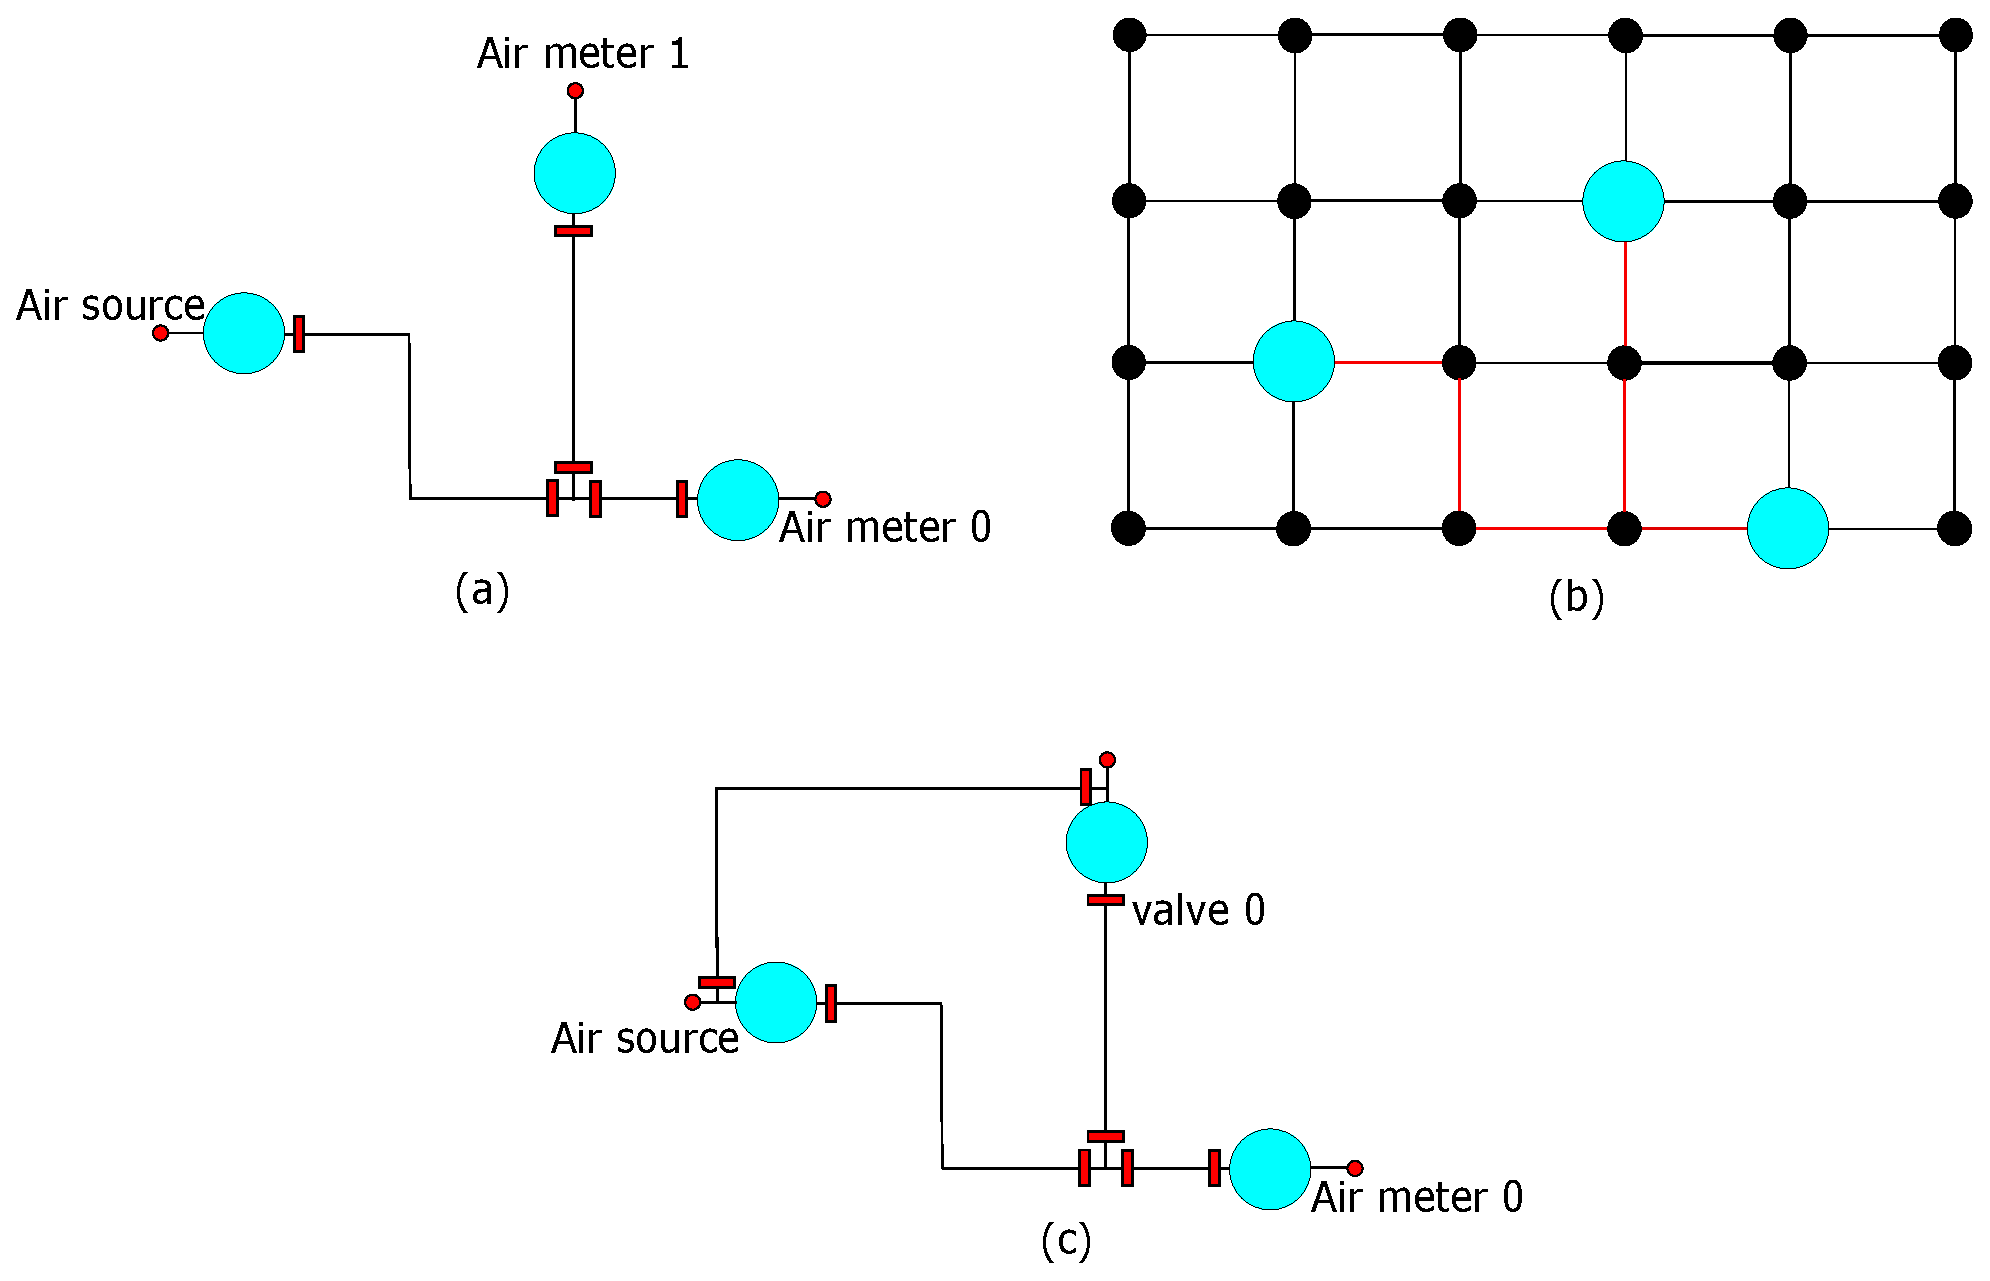
\includegraphics[width=3.50in,height=2.2in]{Fig/fitintogrid2.eps}
\input{Fig/grid.pdf_tex}
\caption{Mapping a biochip onto a virtual connection grid.}
%(a) Origin biochip. (b) Connection grid after mapping. Thick edges 
%represent the edges occupied by the original channels.}
%(c) Design-for-test architecture}
\label{fig:fitintogrid}
\end{figure}


Since the channel segments occupied by the original chip must appear in the new
architecture, the constraints for these edges can be written as
\begin{equation}\label{eq:edge_cover}
\sum_{p_r\in P} e_{j,r}\ge 1,\quad \forall e_j\in E_{o} 
\end{equation}
where $P$ is the set of all test paths; $E_{o}$ is the set 
of edges occupied by the original channels in the connection grid.

When generating the DFT architecture of the chip, we minimize the number of
added channels.
We use a 0-1 variable $s_j$ to represent whether the edge $e_j$ in the connection
grid should be kept in the final chip. If any test path covers $e_j$, $s_j$
must be 1, so that the relation between $s_j$ and $e_j$ can be established as
\begin{equation}\label {eq:edge_used} 
  s_j\ge e_{j,r}, \quad \forall p_r\in P, \quad \forall e_j \in E \backslash E_{o}
\end{equation} 
where $P$ is the set of all test paths and $E \backslash E_{o}$ 
represents the set of edges in the connection grid that are not covered by the original
chip.

Finally, the architecture of the DFT chip can be determined by solving the
following optimization problem
\begin{align} \label{eq:DFT_opt_1}
\text{minimize} & \quad \sum_{e_j\in E\backslash E_{o}}s_j\\
\text{subject to} & \quad
\text{(\ref{eq:path_construct})--(\ref{eq:edge_used})}.\label{eq:DFT_opt_2}
\end{align}

In this optimization, the number of potential test paths $|P|$ should be
determined in advance. This number should be large enough to cover all the
channels in the augmented architecture. In the implementation, we started by
setting this number to 2, and increased it by 1 in the next iteration when the current number
produces no valid result. Another issue is that the formulation above assumes
that starting and ending nodes of paths are given. Although any two ports in
the chip are feasible test ports in the final DFT architecture, we used the
two ports between which the distance is the largest to generate long instead
of short test paths, so that more channels and devices in the original chip
can be covered by an individual path potentially. The last issue of the
formulation above is that loops may be generated on the paths. These loops
need to be excluded to avoid false coverage of the original channels and
devices. In the proposed method, we used the technique in
\cite{LLHS17} to exclude these loops.

%\subsection{Test Vectors and Application Scheduling}

In generating DFT valves and channels above, the test paths to detect
stuck-at-0 defects have been created simultaneously. The stuck-at-1 defects
are detected by test cuts applied to the chip. A cut is composed of a
set of valves which separate the port connected to the pressure source and the
port connected to the pressure meter during test.  After test paths are
created for single-source single-meter test, test cuts can always be created
successfully because in the worst case test paths can be blocked individually
to form cuts. The problem to find the minimum set of test cuts for a given
biochip is a complementary problem of the test path generation
%in Section~\ref{sec:dft_arch} 
so that the details are omitted due the page limit.  



\begin{figure}
\figurefontsize
\centering
%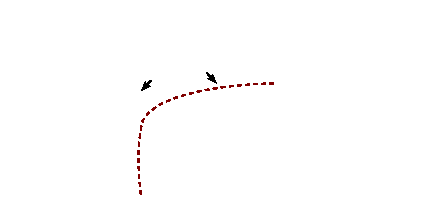
\includegraphics[width=3.00in,height=1.50in]{Fig/valveSharing.eps}
\input{Fig/valveSharing.pdf_tex}
\caption{Valve sharing and its interfering with test and application execution.}
\label{fig:valveSharing}
\end{figure}

\section{Valve Sharing in Test and Application
Execution}\label{sec:valve_sharing}

In implementing single-source single-meter test for a multi-port
biochip, new DFT channels and valves are added into the chip architecture. The
newly added DFT valves also require control signals that switch them open or
closed to regulate the fluid transportation. These control signals are also
air pressure conducted to valves through control channels. If the newly added
DFT valves are controlled independently, both control channels and 
external air pumps should be added, leading to an increase of the cost for manufacturing
and running the chip.  In this section, we propose a valve-sharing technique
which eliminates the control overhead by sharing the control signals of
DFT valves with those for original valves, while maintaining the performance
of the chip.

\subsection{Valve Sharing and its Validation}\label{sec:validation}

Figure~\ref{fig:valveSharing} demonstrates how valves share controlling
channels in a DFT architecture, where each new valve is connected to the
control channel that is already existing to control another valve in the
original chip.  In this example, the DFT valve $v_0$ shares its control
channel with $v_3$ and the DFT valve $v_2$ shares its control channel with
$v_1$.  Consequently, $v_0$ and $v_3$ always open and close simultaneously,
and so do $v_2$ and $v_1$. This sharing scheme, however, interferes with the
test procedure as well as the execution of the application.  Therefore, we
need to develop methods to validate a valve sharing scheme before exploring the
design space of valve sharing.

%\subsubsection{Validation of valve sharing for testing}

Assume that $v_1$ and $v_3$ are kept closed during test to form a cut to
separate the pressure source and the pressure meter.  If $v_3$ cannot be
closed properly due to defects, it is supposed that the pressure 
meter should be able to measure
the leaked air pressure. However, with valve sharing shown in
\figname~\ref{fig:valveSharing}, $v_0$ is also closed, masking the error
supposed to be detected by this cut.

To validate whether a given valve sharing scheme is valid for the test
procedure, each test vector, either a test path or a test cut, is applied
and the output at the pressure meter is verified. For example, in the
case in \figname~\ref{fig:valveSharing}, the validation can be performed
by checking whether there is still a path from the pressure source to the
meter after the test cut is activated and a valve, e.g., $v_3$, cannot be
closed properly. 

Similarly, valve sharing may also affect the execution of an application.
Assume a transportation of fluid is performed from device $d_0$ to device
$d_1$ through the upper path, so that $v_0$ must be opened. However, 
$v_3$ is also opened due to valve sharing, leading to a fluid leakage at $d_1$.

The validation of a valve sharing scheme during application execution is similar
to the case for test. In a given schedule of an application, 
%the device and channel occupation at every moment is known.  
the occupation of all devices and channels at every moment are known. 
These snapshots of
chip occupation are examined together with the given valve sharing scheme
to check whether all the operations can be performed correctly.

\subsection{DFT with Valve Sharing using Particle Swarm Optimization (PSO)}

As discussed above, DFT augmentation brings new channels and valves into
the chip. Not only the locations of added channels and valves but also the
control sharing scheme affect the test procedure and the execution of the
application. In the proposed method, we deploy the Particle Swarm Optimization
(PSO) algorithm to find valid DFT architectures that still maintain the
efficiency of application execution.

Particle swarm optimization (PSO) is a stochastic population-based
optimization algorithm \cite{pso95}. Members of the population (swarm) are
called particles.  At the beginning of the algorithm, particles are randomly
scattered into the whole search space. A particle $p_i$ possesses a position
$x_i$. A random velocity $v_i$ is assigned to particle $p_i$ and a cost
function is applied for each particle to assess the quality of its current
location.  For each particle $p_i$, a local best position $p_{best,i}$ in its
search history is tracked. For the whole swarm, a global best position
$g_{best}$ with the best assessment of all particles is also recorded.  In
each iteration, the new velocity and position of a particle $p_i$ are updated
as follows
\begin{align}\label{eq:pso_update}
v_i = \omega * v_i + c_1*rand_1*(x_i - p_{best,i})+c_2*rand_2*(x_i-g_{best}) \\
x_i = x_i + v_i 
\end{align}
where $\omega$, $c_1$ and $c_2$ are constants to control the search speed.
$rand_1$ and $rand_2$ are two random numbers to incorporate
stochasticity into the search iterations.
%P is the set of all particles. 
After each iteration, the performance at the new position of each particle
and the global assessment are updated.

%PSO makes each particle moves around in the search space, taking advantage of
%the particle’s own experience and the experience of the particle’s neighbours
%or of the whole swarm to guide the search.

%PSO needs a swarm of particles and their initial positions.  
In the proposed method, the
%initial 
position of a particle consists of two parts of information: 1) how to add new channels
to meet the single-source single-meter requirements; 2)
how new valves share control channels with original valves. 
Therefore, we use two multidimensional vectors to denote these positions.
%two parts of information.

In Section~\ref{sec:dft_arch}, the optimization problem
(\ref{eq:DFT_opt_1})--(\ref{eq:DFT_opt_2}) may produce  many viable solutions
to meet the constraints and the objective.
%specially the the minimization objective is  Therefore, we can use different
%edges combination to construct additional channels to meet DFT requirements. 
A vector $\vec{X}^{a}= [x_0,x_1,...,x_n]$ is thus used to denote which edges
in the connection grid are used to construct new channels.  The definition of
$x_i$ is as follows.
\begin{equation}
  x_i =
  \begin{cases}
    1 & \text{if $e_i$ in the connection grid 
      is used for DFT;}\\
    0 & \text{otherwise}
  \end{cases}
\end{equation}
where $e_i$ represents an edge in the connection grid in \figname~\ref{fig:fitintogrid}.
%where $n$ is the number of possible edges to construct a DFT architecture in a connection grid.

%Knowing the locations of new edges added for DFT, we can also deduce the
%locations of valves at the crossing points of channels. 
For valve sharing, assume that the number
of valves for DFT is $n_d$ and the number of valves in the original chip is
$n_v$.  A vector
$\vec{X}^{s}$
is used to denote how DFT valves share control channels with original valves,
defined as
\begin{align}\label{eq:valves_include}
  \vec{X}^{s} =\{x_{i,j}\}, \qquad 0\le i\le n_d, \quad  0\le j\le n_v\\
  x_{i,j}=
  \begin{cases}
    1 & \text{if valve $v_i$ shares control channel with valve $v_j$}; \\
    0 & \text{otherwise.}
  \end{cases}
\end{align}

A PSO particle position is defined as the combination of the two vectors
$\vec{X} = [\vec{X}^{a}, \vec{X}^{s}]$. The quality of a position is evaluated by
two criteria. First, if the locations of DFT channels and valves as well as the
corresponding control sharing scheme cannot pass the validation step described
in Section~\ref{sec:validation}, the quality of this position is set to
$\infty$, meaning that the execution time of the application is so large that
this position is invalid. If this position can pass the validation, its
quality is set to the corresponding execution time of the application at this
position.

In executing the PSO algorithm, valve sharing information can only be obtained
after DFT channels and valves are created. Moreover, the validation of test
and application execution can be performed after the valve sharing scheme is
determined. Only after these steps, the execution time of the application can
be evaluated.  Consequently, multiple phases are required in each PSO
iteration to generate new particle positions and to assess their quality.

In each PSO iteration, for a particle $p_i$ with its position $\vec{X}_i =
[\vec{X}^{a}_i, \vec{X}^{s}_i]$, the operations are as follows. 

\begin{enumerate} 

    %\newlength{\mylength} 
    \setlength\mylength{\parskip}
    \setlength\parskip{-3.5mm}
    %\setlength\itemsep{0.01em}
  \item 

  $\vec{X}^{a}_i$ is updated according to the PSO search strategy, producing a
  new DFT configuration by solving (\ref{eq:DFT_opt_1})--(\ref{eq:DFT_opt_2}).
  \setlength\parskip{\mylength}

  \item 
 % Finding the best share plan in the given $\vec{X^{add}_i}$. In this phase, 
  A sub-PSO algorithm is applied to find the best valve sharing scheme. 
  First, randomized sub-particles with respect to different valve sharing schemes
  are generated. Their positions are set to $\vec{X}^{s}$. 
  Since for each sub-particle, both new channels and valves as well as their
  sharing information are known, we can then assess the quality of these
  positions by validating them using the technique discussed in 
  Section~\ref{sec:validation}. After the sub-PSO algorithm is finished, 
  a valve sharing with the minimum execution time of the application 
  with respect to this sharing scheme is returned. 
  

  \item 

  By combining $\vec{X}^{a}_i$ and its best valve sharing scheme
  $\vec{X}^{s}_i$, we update the quality of the position 
  $\vec{X}_i = [\vec{X}^{a}_i, \vec{X}^{s}_i]$ for $p_i$ with the returned
  application execution time. 

  \item 
    
  After all particles find their new positions and their qualities are assessed,
  the local best position $p_{best,i}$ for particle $p_i$ and the 
  global best position $g_{best}$ are updated accordingly. The iteration goes
  back to step (1) until the maximum allowed number of iterations is reached.

\end{enumerate}

The PSO algorithm returns a DFT architecture together with its valve sharing
scheme. The test vectors and application schedule considering valve sharing
are also generated. The new architecture does not impose
more control overhead, while facilitating the test process and maintaining 
the performance of application execution.

%!!!psuedo code?????

\section{Simulation Results}\label{sec:results}

The proposed framework was implemented in C++ and tested
using a \SI[mode=text]{3.20}{\GHz} CPU with 
\SI{8}{GB} memory.
We demonstrate
the results using FPVAs with valves in different rows and columns. The
tested arrays are shown in Table I, where the first column shows
the dimensions of the arrays and the second column shows
the number of valves. 
We used Gurobi \cite{gurobi} to solve the optimization problems in the
proposed method.

The results of testing FPVAs with a single pressure source and a single pressure sensor
are shown in Table~\ref{tb_test}.
% These arrays contain long channels for transportation and obstacle areas without
% valves. 
%The numbers of valves in the arrays are shown in the column $n_v$.  
%These numbers are calculated by multiplying
%the row number and column number and subtracting
%the number of valves not built due to channels and obstacles.
The direct approach is the method published in \cite{CBBK17}, which
does not use loop relaxation introduced in Section~\ref{sec:loop_relax} for
acceleration. In Table~\ref{tb_test}, the
numbers of test paths are shown in the column $n^d_p$. The CPU time to
generate these patterns is shown in the column $t^d_p$. The columns $n^d_c$ and
$t^d_c$ show the number of cut patterns and the CPU time to generate them.
The columns $n^d_l$ and $t_l^d$ show the number of patterns for testing leakage in the
control layer and the CPU time to generate these patterns. The
total number of test patterns is shown in the column $N^d$. 
``*'' means that no valid results are available 
%from the corresponding approach 
due to runtime.
According to these results, the direct approach suffers from the scalability problem
due to its pure ILP formulation.
%Though the flow path test patterns can still be found with the valve array of
%the size $20\times20$, the cut patterns cannot be generated.
In these results, the number of cuts is much larger than the number of test
paths. This is because a path can travel through many valves in a zigzag shape and 
only a few orthogonal paths can already cover all the valves.
However, the cuts required to cover all the valves in an
FPVA is proportional to the size of the array, leading a much larger number of
such test patterns.

\begin{figure}[t]
{\figurefontsize
\centering
\pgfplotsset{compat=1.3,
    %legend drawing style, single bar instead of the default double mini bars
    /pgfplots/ybar legend/.append style={ 
        /pgfplots/legend image code/.code={%
           \draw[##1,/tikz/.cd,yshift=-0.25em]
           (0cm,0cm) rectangle (5pt,0.8em);
        },
    }
}
\begin{tikzpicture}
\begin{axis}[
% x=1.1cm, y=0.25cm, ymax=12, line width=0.75pt,
x=1.1cm, y=1.40, ymax=55, line width=0.75pt,
xlabel={FPVAs with different size}, xlabel shift=-5pt,
ylabel={Number of test patterns}, ylabel shift=0pt, 
xtick={1,...,6},xticklabels={$5\times5$, $10\times10$, $15\times15$, $20\times20$, $25\times25$, $30\times30$},
x tick label style={rotate=330, xshift=-15pt,yshift=-8pt,anchor=west}, 
xticklabel pos=left, xtick align=outside, xtick pos=left,
ytickmin=0,ytickmax=40,
% ymin = 0,
% ymax = 1,
ytick={0,10,20,30}, yticklabels={0,10,20,30},
legend columns=4, legend style={at={(0.5,0.88)}, anchor=center, nodes={inner xsep=0pt},
draw=none, column sep=5pt},
ybar=0pt, bar width=7
]

   \addplot[line width=0.5pt, black, fill=orange!70!white] table[x=size,y=2port] 
{port_testvector_number.dat};
   \addplot[line width=0.5pt, black, fill=blue!65!orange] table[x=size,y=3port] 
{port_testvector_number.dat};
   \addplot[line width=0.5pt, black, fill=blue!40!orange] table[x=size,y=4port] 
{port_testvector_number.dat};
   \addplot[line width=0.5pt, black, fill=blue!80!orange] table[x=size,y=5port] 
{port_testvector_number.dat};
   \legend{3 Ports\hspace*{0.5pt}, 4 Ports\hspace*{0.5pt}, 5 Ports\hspace*{0.5pt}, 6 Ports\hspace*{0.5pt}}
\end{axis}
\end{tikzpicture}

%\begin{tikzpicture}
\begin{axis}[
% x=1.1cm, y=0.25cm, ymax=12, line width=0.75pt,
x=1.1cm, y=1.40, ymax=60, line width=0.75pt,
ylabel={Cut-set Test Vector Number}, ylabel shift=-6pt, 
xtick={1,...,6},xticklabels={$5\times5$, $10\times10$, $15\times15$, $20\times20$, $25\times25$, $30\times30$},
x tick label style={rotate=330, xshift=-15pt,yshift=-5pt,anchor=west}, 
xticklabel pos=left, xtick align=outside, xtick pos=left,
ytickmin=0,ytickmax=40,
% ymin = 0,
% ymax = 1,
ytick={0,5,10,15,20,25,30,35,40}, yticklabels={0,5,10,15,20,25,30,35,40},
legend columns=4, legend style={at={(0.5,0.9)}, anchor=center, nodes={inner xsep=2pt},
draw=none, column sep=1pt},
ybar=0pt, bar width=7
]

   \addplot[line width=0.5pt, black, fill=orange!70!white] table[x=size,y=2port] 
{port_cut_number.dat};
   \addplot[line width=0.5pt, black, fill=blue!65!orange] table[x=size,y=3port] 
{port_cut_number.dat};
   \addplot[line width=0.5pt, black, fill=blue!40!orange] table[x=size,y=4port] 
{port_cut_number.dat};
   \addplot[line width=0.5pt, black, fill=blue!80!orange] table[x=size,y=5port] 
{port_cut_number.dat};
   \legend{3 Ports\hspace*{0.5pt}, 4 Ports\hspace*{0.5pt}, 5 Ports\hspace*{0.5pt}, 6 Ports\hspace*{0.5pt}}
\end{axis}
\end{tikzpicture}
%%\begin{tikzpicture}
\begin{axis}[
x=1.1cm, y=0.26cm, ymax=12, line width=0.75pt,
ylabel={Exec./Valve Ratio}, ylabel shift=-6pt, 
xtick={1,...,6},xticklabels={RA100, RA70, CPA, RA30, IVD, PCR},
x tick label style={rotate=330, xshift=-15pt,yshift=-5pt,anchor=west}, 
xticklabel pos=left, xtick align=outside, xtick pos=left,
ytickmin=0,ytickmax=10, 
ytick={0,5,10}, yticklabels={0,0.5,1},
legend columns=2, legend style={at={(0.5,0.9)}, anchor=center, nodes={inner xsep=2pt},
draw=none, column sep=1pt},
ybar=0pt, bar width=7
]
   \addplot[line width=0.5pt, black, fill=orange!70!white]
table[x=cir,y=exetime] 
{exe_time_valve_cmp.dat};
   \addplot[line width=0.5pt, black, fill=blue!65!orange] table[x=cir,y=valve] 
{exe_time_valve_cmp.dat};
   \legend{Execution Time\hspace*{9pt}, Valve\hspace*{8pt}}
\end{axis}
\end{tikzpicture}

\caption{Comparison of numbers of test patterns for FPVAs with different
numbers of ports.}
\label{fig:port_test}
}
\end{figure}

\begin{figure}[t]
{\figurefontsize
\centering
\pgfplotsset{compat=1.3,
    %legend drawing style, single bar instead of the default double mini bars
    /pgfplots/ybar legend/.append style={ 
        /pgfplots/legend image code/.code={%
           \draw[##1,/tikz/.cd,yshift=-0.25em]
           (0cm,0cm) rectangle (5pt,0.8em);
        },
    }
}
\begin{tikzpicture}
\begin{axis}[
% x=1.1cm, y=0.25cm, ymax=14, line width=0.75pt,
x=1.1cm, y=9.00, ymax=9, line width=0.75pt,
xlabel={FPVAs with different size},xlabel shift=-5pt,
ylabel={Number of test trees}, ylabel shift=0pt, 
xtick={1,...,6},xticklabels={$5\times5$, $10\times10$, $15\times15$, $20\times20$, $25\times25$, $30\times30$},
x tick label style={rotate=330, xshift=-15pt,yshift=-8pt,anchor=west}, 
xticklabel pos=left, xtick align=outside, xtick pos=left,
ytickmin=0,ytickmax=6,
% ymin = 0,
% ymax = 1,
ytick={2,4,6}, yticklabels={2,4,6},
legend columns=4, legend style={at={(0.5,0.86)}, anchor=center, nodes={inner xsep=0pt},
draw=none, column sep=5pt},
ybar=0pt, bar width=7
]

   \addplot[line width=0.5pt, black, fill=orange!70!white] table[x=size,y=5] 
{hole_wall_path.dat};
   \addplot[line width=0.5pt, black, fill=blue!65!orange] table[x=size,y=10] 
{hole_wall_path.dat};
   \addplot[line width=0.5pt, black, fill=blue!40!orange] table[x=size,y=15] 
{hole_wall_path.dat};
   \addplot[line width=0.5pt, black, fill=blue!80!orange] table[x=size,y=20] 
{hole_wall_path.dat};
   \legend{5\% \hspace*{0.5pt}, 10\% \hspace*{0.5pt},15\%\hspace*{0.5pt},20\%\hspace*{0.5pt}}
\end{axis}
\end{tikzpicture}
\vskip 10pt\pgfplotsset{compat=1.3,
    %legend drawing style, single bar instead of the default double mini bars
    /pgfplots/ybar legend/.append style={ 
        /pgfplots/legend image code/.code={%
           \draw[##1,/tikz/.cd,yshift=-0.25em]
           (0cm,0cm) rectangle (5pt,0.8em);
        },
    }
}
\begin{tikzpicture}
\begin{axis}[
% x=1.1cm, y=0.25cm, ymax=14, line width=0.75pt,
x=1.1cm, y=1.40, ymin=0, ymax=49.5, line width=0.75pt,
xlabel={FPVAs with different size}, xlabel shift=-5pt,
ylabel={Number of cuts}, ylabel shift=0pt, 
xtick={1,...,6},xticklabels={$5\times5$, $10\times10$, $15\times15$, $20\times20$, $25\times25$, $30\times30$},
x tick label style={rotate=330, xshift=-15pt,yshift=-8pt,anchor=west}, 
xticklabel pos=left, xtick align=outside, xtick pos=left,
ytickmin=0,ytickmax=40,
% ymin = 0,
% ymax = 1,
ytick={10,20,30}, yticklabels={10,20,30},
legend columns=4, legend style={at={(0.5,0.86)}, anchor=center, nodes={inner xsep=0pt},
draw=none, column sep=5pt},
ybar=0pt, bar width=7
]

   \addplot[line width=0.5pt, black, fill=orange!70!white] table[x=size,y=5] 
{hole_wall_cut.dat};
   \addplot[line width=0.5pt, black, fill=blue!65!orange] table[x=size,y=10] 
{hole_wall_cut.dat};
   \addplot[line width=0.5pt, black, fill=blue!40!orange] table[x=size,y=15] 
{hole_wall_cut.dat};
   \addplot[line width=0.5pt, black, fill=blue!80!orange] table[x=size,y=20] 
{hole_wall_cut.dat};
   \legend{5\% \hspace*{0.5pt}, 10\% \hspace*{0.5pt},15\%\hspace*{0.5pt},20\%\hspace*{0.5pt}}
\end{axis}
\end{tikzpicture}

%\begin{tikzpicture}
\begin{axis}[
x=1.1cm, y=0.26cm, ymax=12, line width=0.75pt,
ylabel={Exec./Valve Ratio}, ylabel shift=-6pt, 
xtick={1,...,6},xticklabels={RA100, RA70, CPA, RA30, IVD, PCR},
x tick label style={rotate=330, xshift=-15pt,yshift=-5pt,anchor=west}, 
xticklabel pos=left, xtick align=outside, xtick pos=left,
ytickmin=0,ytickmax=10, 
ytick={0,5,10}, yticklabels={0,0.5,1},
legend columns=2, legend style={at={(0.5,0.9)}, anchor=center, nodes={inner xsep=2pt},
draw=none, column sep=1pt},
ybar=0pt, bar width=7
]
   \addplot[line width=0.5pt, black, fill=orange!70!white]
table[x=cir,y=exetime] 
{exe_time_valve_cmp.dat};
   \addplot[line width=0.5pt, black, fill=blue!65!orange] table[x=cir,y=valve] 
{exe_time_valve_cmp.dat};
   \legend{Execution Time\hspace*{9pt}, Valve\hspace*{8pt}}
\end{axis}
\end{tikzpicture}

\caption{Comparison of numbers of test patterns for 
FPVAs with different numbers of long channels and obstacles.}
\label{fig:wall_hole_test}
}
\end{figure}

\begin{table*}[t] 
\centering
{\footnotesize
\renewcommand{\tabcolsep}{10.35pt}
\renewcommand{\arraystretch}{1}
\caption{Comparison between test patterns generated by the proposed method
and the ATPG-based method}
\label{tb_tradition}
\begin{tabular}{ c  c  c c c c c} \hlinewd{0.7pt}
\multicolumn{3}{c}{Proposed method} &
\multicolumn{1}{c}{} &
\multicolumn{3}{c}{ATPG-based method \cite{HuYHC14}}\\
% \multicolumn{1}{c}{} &
% \multicolumn{7}{c}{Acceleration} \\
\cline {1-3}\cline {5-7}
\multicolumn{1}{c}{} &
\multicolumn{1}{c}{Test Pattern} &
\multicolumn{1}{c}{Detected Faults} &
\multicolumn{1}{c}{} &
\multicolumn{1}{c}{} &
\multicolumn{1}{c}{Test Pattern} &
\multicolumn{1}{c}{Detected Faults}\\
% \multicolumn{1}{c}{$n^d_p$} &
% \multicolumn{1}{c}{$t^d_p(s)$} &
% \multicolumn{1}{c}{$n^d_c$} &
% \multicolumn{1}{c}{$t^d_c(s)$} &
% \multicolumn{1}{c}{$n^d_l$} &
% \multicolumn{1}{c}{$t^d_l(s)$} &
% \multicolumn{1}{c}{$N^d$} &
% % \multicolumn{1}{c}{$T^d(s)$} &
% \multicolumn{1}{c}{} &
% \multicolumn{1}{c}{$n^a_p$} &
% \multicolumn{1}{c}{$t^a_p(s)$} &
% \multicolumn{1}{c}{$n^a_c$} &
% \multicolumn{1}{c}{$t^a_c(s)$} &
% \multicolumn{1}{c}{$n^a_l$} &
% \multicolumn{1}{c}{$t^a_l(s)$} &
% \multicolumn{1}{c}{$N^a$} \\
% \multicolumn{1}{c}{$T^a(s)$} \\


\hlinewd{0.6pt}
\hline
1	&0010000011100111110000110000	&17 	&&1	&1111010101100010010110101000	&12\\
2	&1010101110111111001100001101	&5		&&2	&0111001010010111010100010011	&10\\
3	&1011100111111100111111111111	&2		&&3	&1110011110100111100111001111	&13\\
4	&1111111101111111111111111111	&1		&&4	&1110010011101110001110010011	&4\\
5	&1101111111111111111111111111	&1		&&5	&0110100110101110100011110100	&5\\
6	&1111111111011111111101111111	&1		&&6	&1111011010100111110111111000	&5\\
7	&1111111111111011111111111111	&1		&&7	&0010101010110110101101011001	&2\\
8	&1111111011101111111111101111	&24		&&8	&1010011111110101010010011100	&4\\
9	&0010000110111111000000010111	&11		&&9	&0010011010110101110100100010	&1\\
	&								&		&&10	&0011010011011111010000000011	&1\\
	&								&		&&11	&0100101011010101010001001101	&1\\
	&								&		&&12	&1010100111100011100001101011	&1\\
	&								&		&&13	&1011010011110111110000100001	&1\\
	&								&		&&14	&1110001010110111010010011001	&1\\
	&								&		&&15	&1010011011111111101011000100	&1\\
	&								&		&&16	&1011110111101111010011001000	&1\\


\hline



% 5  $\times$ 5   &39  &&1 $\times$  1&5 $\times$ 5  &&5  & 0.3  &&8  &0.2 & &  4  &  2   &&17 & 2.5 \\ 
% 10 $\times$ 10  &176 &&2 $\times$  2&5 $\times$ 5  &&4  & 4    &&18 &5   & &  4  &  10  &&26 & 19  \\
% 15 $\times$ 15  &411 &&3 $\times$  3&5 $\times$ 5  &&8  & 17   &&28 &26  & &  8  &  127 &&44 & 170 \\
% 20 $\times$ 20  &744 &&4 $\times$  4&5 $\times$ 5  &&16 & 35   &&38 &41  & & 16  & 742  &&70 & 818 \\
% 30 $\times$ 30  &1704&&6 $\times$  6&5 $\times$ 5  &&20 & 255  &&58 &171 & & 20  & 1492 &&98 & 1918\\
\hlinewd{0.7pt}
\end{tabular}
}
\end{table*}











%finding
%cuts without any acceleration method is thus infeasible due to the nature of
%ILP formulation.

The columns of loop acceleration show the results of generating test patterns using
loop relaxation. The columns $n^a_p$, $n^a_c$ and $n^a_l$ show the
numbers of test paths, cuts and leakage test patterns,
respectively.
The columns $t^a_p$, $t^a_c$ and $t^a_l$
show the CPU time needed to generate these patterns, respectively. The total number
of the test patterns is
shown in the column $N^a$. These results show that with loop acceleration 
valid test patterns can be generated for all these valve arrays, though the CPU
time increases quickly as the size of the FPVA grows.
%\textbf{For the test case $15\times15$, one extra flow path is required in the
  %loop acceleration method, due to the heuristic nature of this acceleration
  %technique. BUT IN THE RESULTS THE NUMBERS OF THE PATH TEST PATTERNS ARE THE
%SAME?} 
%. When generating cut-set test vectors,
%because the number of cuts increases with the size of the FPVA , additionally
%to Lagrangian relaxation, we generate one cut at a time to cover as many valves
%as possible. This is reason why the execution time for generating cuts is
%significantly shorter than that of the direct approach. 
For the case 30$\times$30, 
the numbers of variables and constraints 
in the ILP formulation
for generating the test patterns to detect stuck-at-0 faults, 
stuck-at-1 faults and control-layer leakage are already (17702,36910), 
(100920,1016247) and (20511,88552), respectively. 
Therefore, a long CPU time
was required to solve the corresponding optimization problems.

The results of the proposed method for multiple-port test is shown in
\figname~\ref{fig:port_test}, where 
%.  In \figname~\ref{fig:port_test}(a), 
the numbers of total test patterns for FPVAs with different numbers of test ports
are compared. 
With this comparison, it can be seen that the number of test
patterns decreases quickly as the number of test ports increases. 
This is also valid when the number of test patterns with three ports is compared
with that with two ports shown in Table~\ref{tb_test}.
Since the majority of the test patterns are cuts,
more test ports enable a better coverage of valves by cuts composed of multiple
segments,
%as shown in Fig~\ref{fig:port_test}(b).
leading to a significant reduction of test patterns.

We also 
demonstrate the effectiveness of our method in dealing with long channels
and obstacles in FPVAs. The results are shown in
\figname~\ref{fig:wall_hole_test}. In these cases, we randomly
created FPVA layouts with 5\%, 10\%, 15\% and 20\% missing valves and
obstacles. For each of these cases, one pressure source and two pressure sensors are 
assumed.
As shown in this comparison, long channels and obstacles 
have only slight influence on the number of test patterns for FPVA test.
%makes little
%difference on the number of trees and cuts needed to test all vavles, as shown
%in Fig~\ref{fig:wall_hole_test}.
However, it is worth noting that the real form of the test trees and cuts are
completely different from those without long channels and obstacles. 

We have applied the proposed method onto the traditional multiple-port
continuous-flow biochip shown 
in \figname~\ref{fig:test_traditional} from \cite{HuYHC14}. The port $P3$
is connected to a pressure source. The ports $P1-P2$ and $P4-P15$ are connected
to pressure sensors. 
Table~\ref{tb_tradition} shows the comparison between the test patterns generated by our
method and the test patterns generated by the ATPG method in \cite{HuYHC14} in
detecting stuck-at-0 and stuck-at-1 faults.
The test patterns define the open/closed states
of valves in the order (a--z, A, B), and the numbers of
individual faults that can be detected by the corresponding test patterns are
also shown in the corresponding rows in Table~\ref{tb_tradition}.
The proposed method covers all stuck-at-0 and stuck-at-1 faults with 9 test patterns. 
With the method of converting the same biochip architecture into a circuit 
and then applying ATPG to generate test patterns as proposed in \cite{HuYHC14}, 
16 test patterns are needed. Therefore, the method proposed in this paper has a
better efficiency in fault coverage. 
%a 78\% increase compared to our method. 


 \begin{figure}[t]
 {\figurefontsize
 \centering
 \input{Fig/test_traditional.pdf_tex}
 \caption{A traditional multiple-port continuous-flow biochip from \cite{HuYHC14}. P1-P15 are ports. a-z, A and B are valves.}
 \label{fig:test_traditional}
 }
 \end{figure}

\begin{figure*}
{\figurefontsize
\centering
\input{Fig/kill_loops_example.pdf_tex}
\caption{Constructing test trees on a \text{20$\times$20} FPVA with long
channels and obstacles. (a) The original FPVA represented by a graph. (b) Long
channels and obstacles are compressed into super cells. (c), (d) and (e) Three test trees
with a loop in (e).
(f) The previously constructed test tree in (e) is altered to partially
cover the valves on the loop. (g) The remaining valves to cover. (h) One
additional test tree to cover the remaining valves.}
\label{fig:kill_loops_example}
}
\end{figure*}
 
To demonstrate the process of
 tree construction, the intermediate results of the \text{20$\times$20} FPVA
with long channels and obstacles are shown in \figname~\ref{fig:kill_loops_example}. 
The FPVA has been abstracted into a graph, where nodes represent the
cells and edges represent the valves. Randomly generated long channels and obstacles are
created in the array. 
\figname~\ref{fig:kill_loops_example}(a) shows the structure of the original
FPVA, where the red edges represent always-closed valves or 
obstacles. The blue edges represent normal valves that are expected to be
closed and opened during assay execution.
\figname~\ref{fig:kill_loops_example}(b) is the FPVA with its long channels and
obstacles merged 
%into regular cells with the method introduced in
as described in Section~\ref{sec:walls_holes}. \figname~\ref{fig:kill_loops_example}(c), \figname~\ref{fig:kill_loops_example}(d) and \figname~\ref{fig:kill_loops_example}(e) are
the test trees constructed using the ILP model 
%\text{(\ref{eq:ilp_tree_1})-(\ref{eq:ilp_tree_2})} 
with loop relaxation. There is a disjoint loop in \figname~\ref{fig:kill_loops_example}(e) and it is altered  
in \figname~\ref{fig:kill_loops_example}(f).
\figname~\ref{fig:kill_loops_example}(g) shows the remaining valves that need
to be covered by additional trees
after the loop is altered. In \figname~\ref{fig:kill_loops_example}(h), one
additional test tree is constructed to cover these valves.

To verify whether the test paths, cuts and the patterns for testing control
layer leakage can detect faults reliably, for each FPVA in
Table~\ref{tb_test} we generated one, two, three, four and five faults
separately and tested whether the test patterns can detect these faults. We
repeated this process for \num[mode=text]{10000} times.  In these test cases,
the test patterns detected all the faults, 
%meaning that these test patterns are very effective in detecting faults.
%compared with the in-theory guaranteed two-fault detection. 
demonstrating a very high reliability in fault detection.


\section{Conclusion}\label{sec:conclusion}

In this paper, we have proposed the first strategy to generate
test patterns with paths and cuts for fully programmable valve
arrays (FPVAs) to detect faults such as blockage and leakage in the flow
layer and the control layer. The method produces an efficient test set and
can handle a vast majority of flow-based networks that can be
configured on such an array.
In the multiple-port test scenario, these patterns are expanded accordingly to take
advantage of multiple pressure sensors to improve test efficiency.
%we introduce a method to construct test trees and test cuts
%to help generate the test patterns. 
%The number of test vectors from the proposed method is roughly linear to the square
%root of the number of valves, much smaller than the number of test vectors 
%when each valve is tested individually.  
The proposed method can guarantee 
the detection of any two faults in FPVAs, while multiple faults can
actually be captured effectively. 
When applied to traditional flow-based biochips,
the generated patterns also demonstrate a high test efficiency. Identifying the
location of faults in programmable array-based biochips may be investigated
as a future research problem. Selective placement of test ports for
further reduction of test sets is another open problem to study.


\section*{Acknowledgment}

	%\fontsize{8pt}{1}\selectfont
The work of B. Li and U. Schlichtmann was supported by the IGSSE Project FLUIDA of
Technical University of Munich. 
The work of Chunfeng Liu was supported fully, and the work of 
T.-Y. Ho was supported in part, by the Technical University
of Munich -- Institute for Advanced Study, funded by the German
Excellence Initiative and the European Union Seventh Framework Programme under
grant agreement n$^\circ$ 291763.
%The work of T.-Y. Ho was also supported in part by the Ministry of Science and Technology of
%Taiwan, under Grant MOST 105-2221-E-007-118-MY3.





%\let\oldthebibliography=\thebibliography
%\let\endoldthebibliography=\endthebibliography
%\renewenvironment{thebibliography}[1]{%
%\begin{oldthebibliography}{#1}%
%%\setlength{\itemsep}{0ex}%
%%\def\baselinestretch{1}
%\fontsize{8.0pt}{1}\selectfont
%\vskip 1pt
%\scriptsize
%\small
%\footnotesize
%\reffontsize
%\newlength{\mylength}
%\setlength{\mylength}{7.5pt}
%\setlength{\baselineskip}{\baselinestretch\mylength}
%\setlength{\baselineskip}{30pt}
%}%
%{%
%\end{oldthebibliography}%
%}


%%\renewcommand{\baselinestretch}{2} 
\let\oldthebibliography=\thebibliography
\let\endoldthebibliography=\endthebibliography
\renewenvironment{thebibliography}[1]{%
\begin{oldthebibliography}{#1}%
\vspace{3pt}
%%\setlength{\parskip}{0ex}%
%\setlength{\itemsep}{0ex}%
%%%%%%bil
\fontsize{7.0pt}{1}\selectfont
%%\vskip 1pt
%\scriptsize
%%\small
%\reffontsize
}%
{%
\end{oldthebibliography}%
}

%\bibliographystyle{abbrv}
%\bibliographystyle{unsrt}


\bibliographystyle{IEEEtran}
%\bibliographystyle{ACM-Reference-Format}
\bibliography{IEEEabrv,CONFabrv,bibfile}

\end{document}


